\subsection{Periodic Water Cycling Code}

%\minisec{Sketch 1: A flashing LED on a protoboard}

\begin{lstlisting}[style=Arduino, caption=Water Cycle First Code, label=lst:water1]
 /*  Emits a periodic signal one quarter per hour */

// Which pin is connected with the water pump?
const int waterPumpPIN = 4;

// Time intervals
// 15 min = 60e3 ms * 15 = 9e5 ms
const int fifteenMin = 900000;
const int fourtyFiveMin = 2700000;

void setup(){
  // Sets the waterPumpPIN as the output of the periodic signal
  pinMode(waterPumpPIN, OUTPUT);
}

void loop(){
  digitalWrite(waterPumpPIN, HIGH); // sets the signal to logical 1 ON
  delay(fifteenMin); // stay on high voltage for 15 minutes
  digitalWrite(waterPumpPIN, LOW); // sets the signal to logical 0 OFF
  delay(fourtyFiveMin); // stay on low voltage for 45 minutes
}
\end{lstlisting}

% Make a second code based on https://www.arduino.cc/en/Tutorial/BlinkWithoutDelay
\subsubsection{Reviewed Code}
A program that uses delay in the main loop to make timed actions is error-prone,
since the delay will be belated by the overhead of other operations located inside the main loop.
Moreover the Arduino will not detect any interruption during a delay,
so we need to use delays only when it is really necessary.

To make a better code and to improve the scalability of the automation for more use cases that needs to be precisely timed,
one needs to review the code to find another way to do periodic actions.
We used \cite{arduinoDelay} as a reference to remove the delay-based code from water cycling's code \ref{lst:water1}.
Given that Arduino only offers a functions that retrieve time in order of milliseconds,
the listing \ref{lst:wcReview} uses the millis() function.

\begin{lstlisting}[style=Arduino,
                    caption=Water Cycle Code without Delays,
                    label=lst:wcReview]

 /*  Emits a periodic signal one quarter per hour without using delay */

// Which pin is connected with the water pump?
const int waterPumpPIN = 4;

// State of the signal
int waterPumpState = LOW;

// Using unsigned variable to support more data
unsigned long previousMillis = 0; (*@ \label{lst:long} @*)

// Time intervals
// 15 min = 60 s * 15 = 9e3 s
const int fifteenMin = 9000;
unsigned long previousSeconds = 0;
// Milliseconds in one second
const int second = 1000;
// Seconds in one hour
const int hour = 3600;

void setup(){
  // Sets the waterPumpPIN as the output of the periodic signal
  pinMode(waterPumpPIN, OUTPUT);
}

void loop(){
  // Get current time in milliseconds
  unsigned long currentMillis = millis();

  // If a second passes
  if (currentMillis - previousMillis >= second) {
    // Store the last timestamp for the last second
    previousMillis = currentMillis;
    // Increment the number of seconds passed
    ++previousSeconds;
    // Reset each hour
    previousSeconds (*@\%= hour@*);
  }

  // For 15 minutes do
  if ( previousSeconds <= fifteenMin ) {
    digitalWrite(waterPumpPIN, HIGH); // sets the signal to logical 1 ON
  }
  // For other 45 minutes do
  else {
    digitalWrite(waterPumpPIN, LOW); // sets the signal to logical 0 OFF
  }
  
}
\end{lstlisting}

Note that we are storing the timestamps in a 32-bit variable at line \ref{lst:long},
so the overflow will occur in almost 50 days,
because the variable storage limit is $ ( 2^{32} -1 ) $ ms.
\begin{align}
    limit& = FFFF& limit+1& = 0000 \label{overflow}
\end{align}
The overflow phenomenon is showed in \eqref{overflow},
when 4 bytes can't afford to represent larger numbers anymore,
because all bits are set to 1.
If someone adds one to this limit,
the value turns to zero,
due to the 9th bit, or the carry, is ignored.

But there is a fancy property with this overflow that soothes this worry:
the subtraction of two timestamps will remain correct even if there is a overflow in those numbers,
given that the variable is unsigned.
\begin{align}
    time_A &=limit - 3\;milliseconds =FFFB  \label{timeA} \\ 
    time_B &= 10\;milliseconds =000A =limit + B  \label{timeB} \\ 
    time_B - time_A &= 000A - FFFB =000E =14\;milliseconds \label{difference}
\end{align}

For example,
$time_A$ \eqref{timeA} is a timestamp that records a time 3 milliseconds past the overflow,
$time_B$ \eqref{timeB} records a time with 10 milliseconds after overflow,
or 11 milliseconds after the limit,
so there is a difference of 14 milliseconds between $time_B$ and $time_A$.
The equation \eqref{difference} shows that the result is still correct even after an overflow.

\subsection{Finite State Machine}
When a program counts time like the listing \ref{lst:long},
with many conditionals waiting for some event,
such as a time limit,
this program could be interpreted as an implementation of a finite state machine,
or FSM.

\begin{figure}[h]
    \centering
    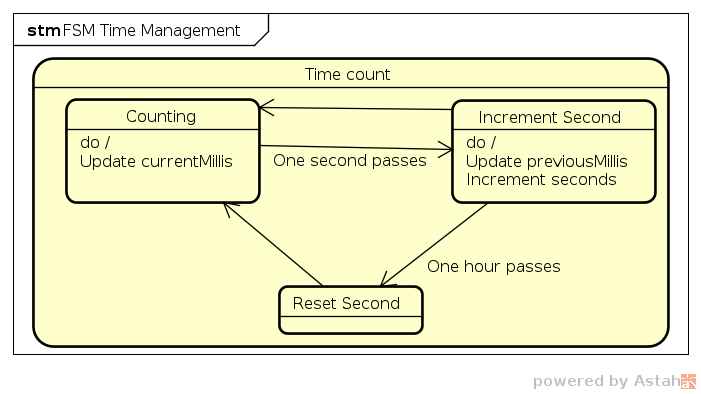
\includegraphics[width=.7\textwidth]{diagrams/FSM_TM.png}
    \caption{A FSM shows how the time counting from periodic water cycle works}
    \label{fig:fsm_tm}
\end{figure}

This representation will be important to design the next requirements,
since we could use the time management FSM to interact with more FSMs.
So this project will be event-driven,
resembling what happens in a real-world environment.

\subsection{pH Level Control}
    If the water tank's pH level is under 6,
    the high pH water will be pumped precisely,
    until the former gets the pH between 6 and 7.
    Or else,
    if the pH reaches levels greater than 7,
    deposit the low pH water in to the tank.

\begin{figure}[h]
    \centering
    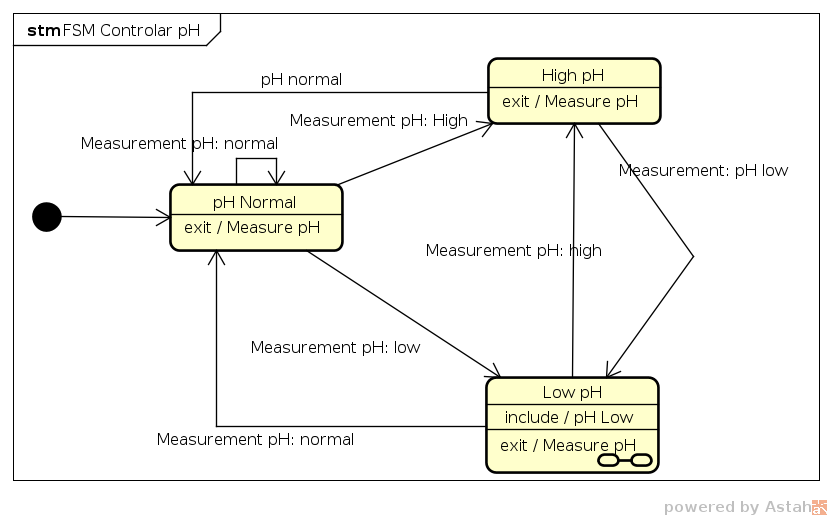
\includegraphics[width=.7\textwidth]{diagrams/pH_Control}
    \caption{A FSM to represent how the system keeps the pH at secure levels}
    \label{fig:fsm_pHc}
\end{figure}

\begin{Code}
    \centering
    \begin{lstlisting}[style=Arduino, caption=pH Control First Code, label=lst:ph1]
    /*  Keeps pH level around 6.5 */

    // Which pin is connected with the pH Sensor?
    const int pHsensorPIN = 5;
    // Which pins are connected with the pH peristaltic pumps?
    const int high_phPIN = 6;
    const int low_phPIN = 7;

    // pH Limits
    const int lowestPH = 6;
    const int highestPH = 7;

    void setup() {
        // Sets the pHsensorPIN as the output
        pinMode(pHsensorPIN, OUTPUT);
    }

    void loop() {
        pHRawValue = analogRead (pHsensorPIN);
        // Transform raw value into the actual one
        pH = process(pHRawValue);

        if ( pH < lowestPH ) {
            // Turning on the high pH pump
            digitalWrite ( high_phPIN, HIGH );
            // Guaranteeing that the low pH pump is off
            digitalWrite ( low_phPIN, LOW );
        }
        else if ( pH < highestPH ) {
            // Turning on the high pH pump
            digitalWrite ( high_phPIN, LOW );
            // Guaranteeing that the low pH pump is off
            digitalWrite ( low_phPIN, HIGH );
        }
    }
    \end{lstlisting}
\end{Code}

